\section{Processen i detaljer\label{ref::process}}

Denne sektion afdækker det flow der ligger til grund for hvorledes det kan bevises at målinger kan foretages under kontrollerede forhold. Derudover er der beskrevet de individuelle faser for hvorledes billedet er behandlet samt hvilke algoritmer der er i brug.\\Det antages at læseren har et grundlæggende kendskab til de nævnte algoritmer.

Formålet er at dokumentere semantikken bag processen, således at det er muligt at kunne genskabe det samme resultat ud fra denne information på anden vis.\\
Der er set bort fra detaljer der er specifikke for implementeringen, med undtagelse for at illustrere eksempler.
For implementering af følgende, henvises til Bilag A, lokaliseret i filen MANGEL!!!!!! 

\subsection{Lysproblematikken}
I den eksisterende iteration af stribemålingen bliver kameraets eksponering kontrolleret i hver fase. Det er for at sikre at målingen kan foretages under skiftende lysforhold, da selv lysforskellen fra når en sky passerer ind foran solen påvirker enten at det ikke er muligt at lokalisere vejstriben eller har indflydelse på resultatet i en sådan grad at det er umuligt at verificere dataen.
Alle faser løser problematikken med skiftende ambient lysforhold ved selv at tage kontrollen over kameraets eksponering og derved finde den optimale længde.\\

\subsection{Lokalisering af striben\label{ref::stribefind}}
Det første problem er at kunne identificere hvor i billedet vejstriben er lokaliseret. Det er en kritisk fase og har ligget til grund for de fleste problematikker som helhed.
\\
Billedet bliver foldet med en diagonal kernel, der sørger for at fremhæve stribens afgrænsninger, der består af to skrå kanter.
Derefter bliver en regulær edge detection, i dette tilfælde Canny, udført på det resulterede billede. For at finde striben på det resulterende billede, benyttes houghlines algoritmen, hvor en afgrænsning i et bestemt antal grader er fastsat. Kriterierne for hvorvidt den mener den har lokaliseret striben er sat ud fra houghlines resultaterne. Houghlines lokaliserer typisk en mængde linjer der vil, grundet stribens kant, være lokaliseret oven i hinanden, i to klumper, i hver sin side af striben.
Ved at verificere at hver første linje i hver klump skærer med de andre linjer i samme klump, kan der med rimelig sikkerhed konstateres at striben er lokaliseret.
\\
Ud fra lokationerne af de to sider, dannes et område der afgrænser kanterne af striben. Området benyttes til at danne afgrænsninger af de tre hovedområder, hvor striben er og hvor den ikke er.

\begin{figure}[h]
	\centering
	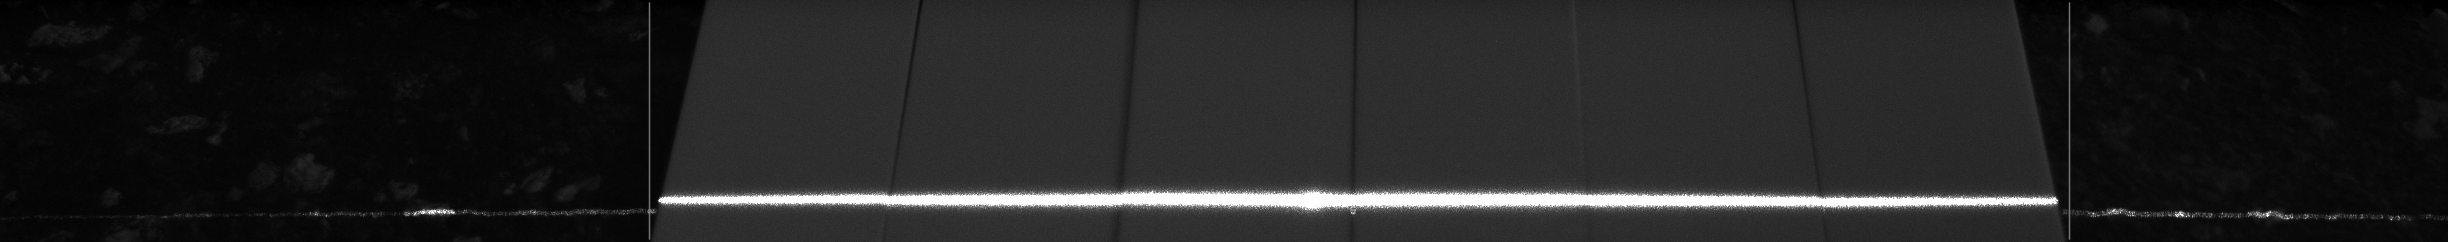
\includegraphics[width=0.8\linewidth]{Billeder/_1_normal}
	\caption{Stribens lokation}
	\label{fig:1normal}
\end{figure}

\newpage

\subsection{Laseren uden for striben}

\begin{figure}[h]
	\centering
	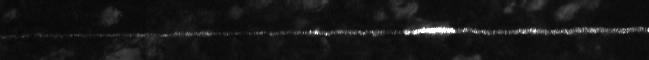
\includegraphics[width=0.7\linewidth]{Billeder/base_1_filter}
	\caption{Laseren uden for striben, filtreret}
	\label{fig:base_1_filter}
\end{figure}

Ved brug af det afgrænsede område fra sektion \ref{ref::stribefind}, antages det at laseren vil befinde sig i den nederste kvarte del af billedet. Hvis det ikke er tilfældet, er lokationen af måleenheden i forhold til striben ikke egnet til at måle fra.
Når afgrænsningen er foretaget, bliver området filtreret med et filter der hjælper med at lokalisere laseren via en hertil valgt kernel. Her illustreret af figur \ref{fig:base_1_filter}.

\begin{figure}[h]
	\centering
	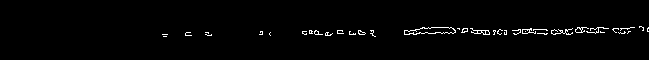
\includegraphics[width=0.7\linewidth]{Billeder/base_2_canny}
	\caption{Lasere efter edge detection}
	\label{fig:base_2_canny}
\end{figure}

Herefter bliver dataen manipuleret i samme stil som i sektion \ref{ref::stribefind}.

Grundet det faktum at laserens repræsentation ved siden af striben ikke er så tydelig, bliver billedet herefter behandlet via en gradient morphology algoritme, der sørger for at lukke små huller ud fra Canny algoritmens resultat.

\begin{figure}[h]
	\centering
	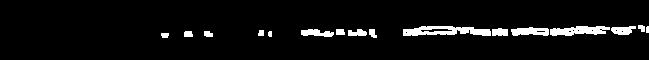
\includegraphics[width=0.7\linewidth]{Billeder/base_3_morph}
	\caption{Lasere efter gradient morphology}
	\label{fig:base_3_morph}
\end{figure}

På dette punkt er informationerne tilstrækkelig rige til at kunne benytte en properlistisk houghlines algoritme til at lokalisere det område hvor laseren befinder sig.

\begin{figure}[h!]
	\centering
	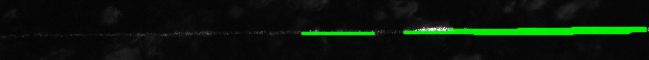
\includegraphics[width=0.7\linewidth]{Billeder/base_4_houghP}
	\caption{Houghlines finder linjer}
	\label{fig:base_4_hough}
\end{figure}

Ud fra de informationer der bliver dannet via houghlines, kan laseren komplette område rammes ind. Herefter følger en vægtning af det indrammede information der er beskrevet mere detaljeret i sektion \ref{ref::weight}.

\subsection{Laseren på striben}
Informationerne i den del af billedet er temmelig anderledes, grundet laserens placering oven på vejstriben. Derfor kan der tages udgangspunkt i den originale eksponering da denne var den lavest mulige til at kunne identificere vejstriben. Det resulterer i at selve laseren vil have en meget høj intensitet i forhold til resten, og det udnyttes til at kunne adskille den position hvor den er ret nemt. Laserens billede bliver udglattet for at modvirke eventuelle mindre overlapninger fra laser til stribe i intensitet hvor det ikke ville være muligt at identificere hvad der hører til laseren og hvad der hører til striben. Når antagelsen af hvor laserens lokation er fundet, bliver dennes data også positionsvægtet, hvilket er beskrevet i sektion \ref{ref::weight}.

\subsection{Vægtet placering\label{ref::weight}}
Algoritmen benytter sig af moments, og mere specifikt \texttt{m01} og \texttt{m00} til at udregne vægtningerne.
Den opbygger en liste af punkter, hvor alle X-koordinaterne befinder sig i stigende orden fra 0 til N, hvor N i dette tilfælde er bredden af det billede den skal bearbejde.
Y-koordinaterne bliver sat ud fra det billede der skal bearbejdes. Den vil opdele billedet i små bidder der er præcis 1 pixel bred, og derefter udfører moments algoritmen på hver af disse bidder. Det resulterer i en enkelt værdi, der er det vægtede punkt i Y, for lige præcis den X. Denne Y-værdi bliver indsat i punktlisten og derved indeholder listen en komplet vægtning i Y for pixel intensiteter, for alle X i et givent billede. Meta data, der omhandler den reale lokation for den udregnede punktliste, bør opbevares andet steds.

\begin{figure}[h]
	\centering
	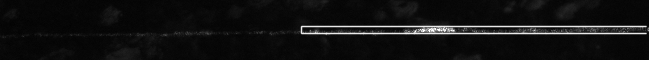
\includegraphics[width=0.7\linewidth]{Billeder/base_5_boxing}
	\caption{Det område der skal udføres intensitetsbaseret vægtning af laseren}
	\label{fig:base_5_boxing}
\end{figure}

\subsection{Højden}
Alt ud fra hvorledes højden ønskes beregnet, f.eks. gennemsnit af de fundne lokationer, kan de gemte data udregnes på den ønskede måde. Dataen i dens rå form åbner op for, at på forskellig vis kunne behandle dem, og opnå de informationer man ønsker.

